\documentclass[UTF8]{ctexart}
\usepackage{graphicx}
\graphicspath{{img/}} 
\title{Homework\ 9}
\author{PB17111623}
\author{PB17111623 范睿}
\date{\today}
\usepackage[a4paper,bottom=3.5cm]{geometry}
\usepackage{algorithm}  
\usepackage{algorithmicx}
\usepackage{amsmath}  
\usepackage{algpseudocode}  %算法的包
\usepackage{amssymb}
\algdef{SE}[DOWHILE]{Do}{doWhile}{\algorithmicdo}[1]{\algorithmicwhile\ #1}%写do-while的话加上这句话
\begin{document}
\maketitle
\section{}
\subsection{子图同构问题取两个无向图 G1 和 G2, 要回答 G1 是否与 G2 的一个子图同构这一问题。证明:子图同构问题是 NP 完全的。}
证明子图同构问题是NP完全的$\Leftrightarrow$子图同构问题既是NP问题,又是NP-hard问题。\\
设$G_1=(V_1,E_1),G+2=(V_2,E_2)$\\\\
1.证明子图同构问题是NP问题:\\
若$G_1$与$G_2$的某一子图$\hat{G_2}=(\hat{V_2},\hat{E_2})$同构,即存在一个映射$f:V_1\rightarrow \hat{V_2}$,若$(u,v)\in E_1\Leftrightarrow \{f(u),f(v)\}\in \hat{E_2}$。若验证此映射$f$是满足同构要求的映射,则遍历$G_1$所有边$(u,v)$,验证$(f(u),f(v))$是否属于$\hat{E_2}$。时间为$\mathcal{O}(E_1)$。因此子图同构问题是NP问题。\\\\
2.证明子图同构问题是NP-hard问题:\\
利用Clique问题为NP-hard问题的结论来证明子图同构问题是NP-hard问题,可以将子图同构问题转化成Clique问题。\\
我们想在$G_2$中找到一个子图,此子图与$G_1$同构,那么我们可以现在$G_2$中找到一个大小为$|V_1|$的团,如果存在这样的团,那么这个团一定与$G_1$同构(相当于找到了与把$G_1$补全成的完全图同构的子图)。此转换时间为$\mathcal{O}(E_1)$,时间为线性。转化后的问题的结果就是原问题的结果,时间也$\mathcal{O}(1)$,因此子图同构问题是NP-hard问题。
\section{证明:哈密顿路径问题是 NP 完全的}
哈密顿路径是经过图中每个顶一次的路径。\\\\
1.证明哈密顿路径问题是NP问题:\\
若存在一条哈密顿路径p,我们可以沿着路径查看。每经过一个顶点将此顶标记为visited,每一个新遇到的顶点都没有被visit过,那么此路径就是一条哈密顿路径,验证时间为$\mathcal{O}(|p|)$。\\\\
2.证明哈密顿路问题是NP-hard问题:\\
利用3SAT问题是NP-hard问题的结论来证明,将3SAT问题转换为哈密顿路径问题。\\
设一个3-CNF的表达式为
\begin{center}
$\Phi=(a_1\lor b_1\lor c_1)\land(a_2\lor b_2\lor c_2)\land...\land(a_k\lor b_k\lor c_k)$
\end{center}
其中,$a_i,b_i,c_i$可以为$x_i$或$\bar{x_i}$。\\
在转化后的图中,将每一个变量用一个钻石形状的子图来代表:\\
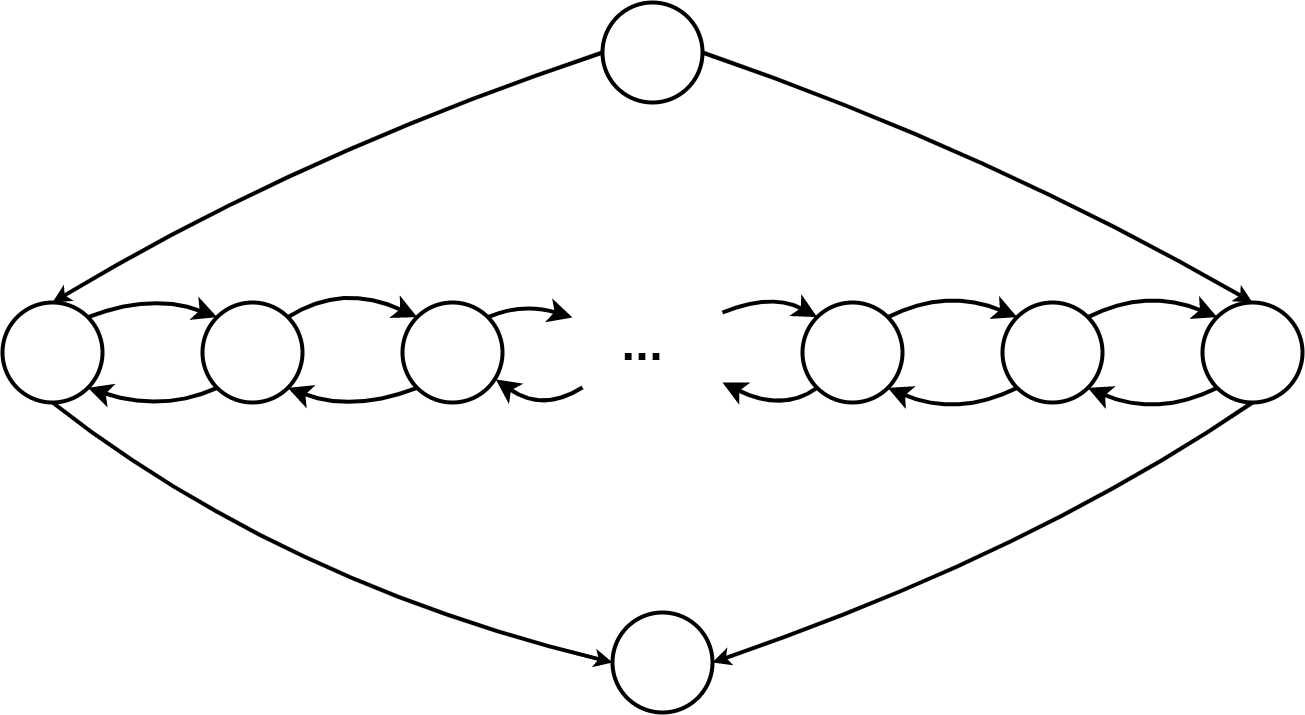
\includegraphics[scale=0.2]{1.png}\\
若表达式中有k个clause,那么钻石形状子图中的中间一行共有3k+1个结点,其中有2k个结点对应着k个clause,k-1个结点将他们连接起来,加上两端的两个结点,共有3k+1个结点:\\
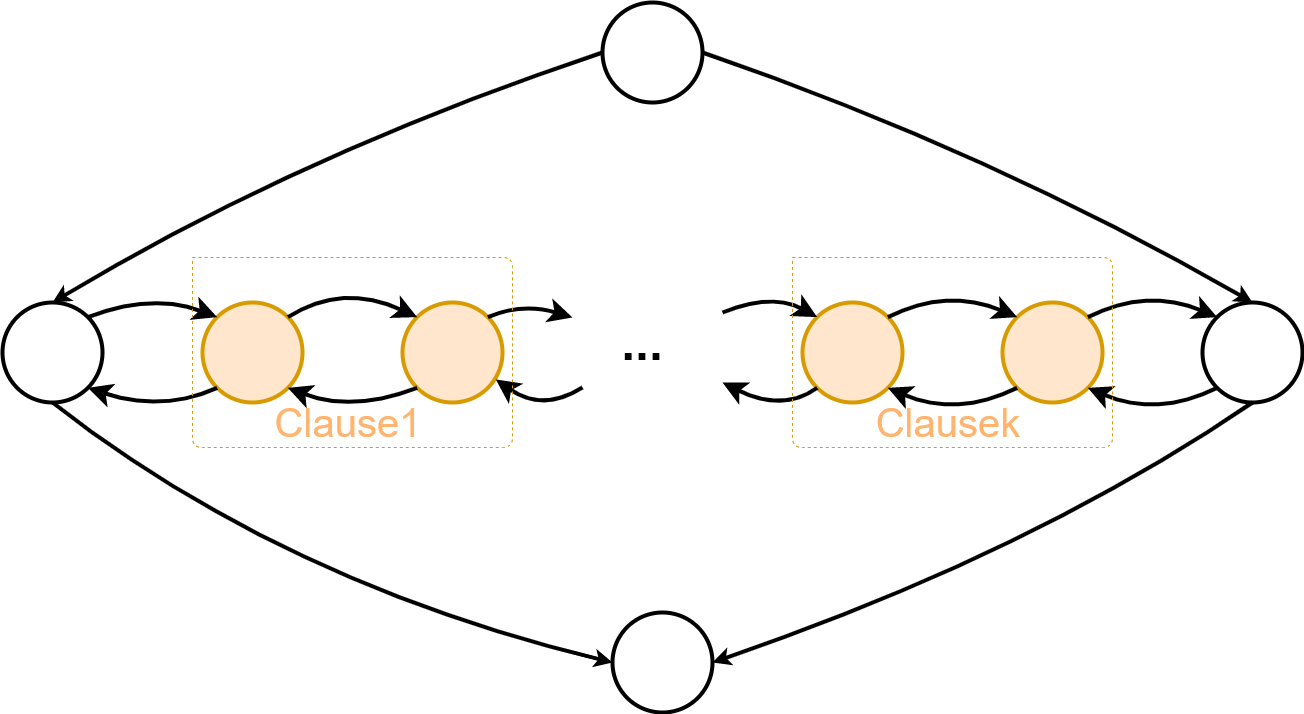
\includegraphics[scale=0.2]{2.png}\\
对每个clause还有一个对应的结点$C_1,C_2,...,C_k$,那么有表达式生成的图G形如:\\
其中,若$x_i$在第j个clause以$x_i$的形式出现,那么第i个钻石子图中的代表与$C_j$相关联的两个结点,左边的指向$C_j$结点,右边的被$C_j$结点指向,否则($x_i$在第j个clause以$\bar{x_i}$的形式出现),第i个钻石子图中的代表与$C_j$相关联的两个结点,右边的指向$C_j$结点,左边的被$C_j$结点指向。\\
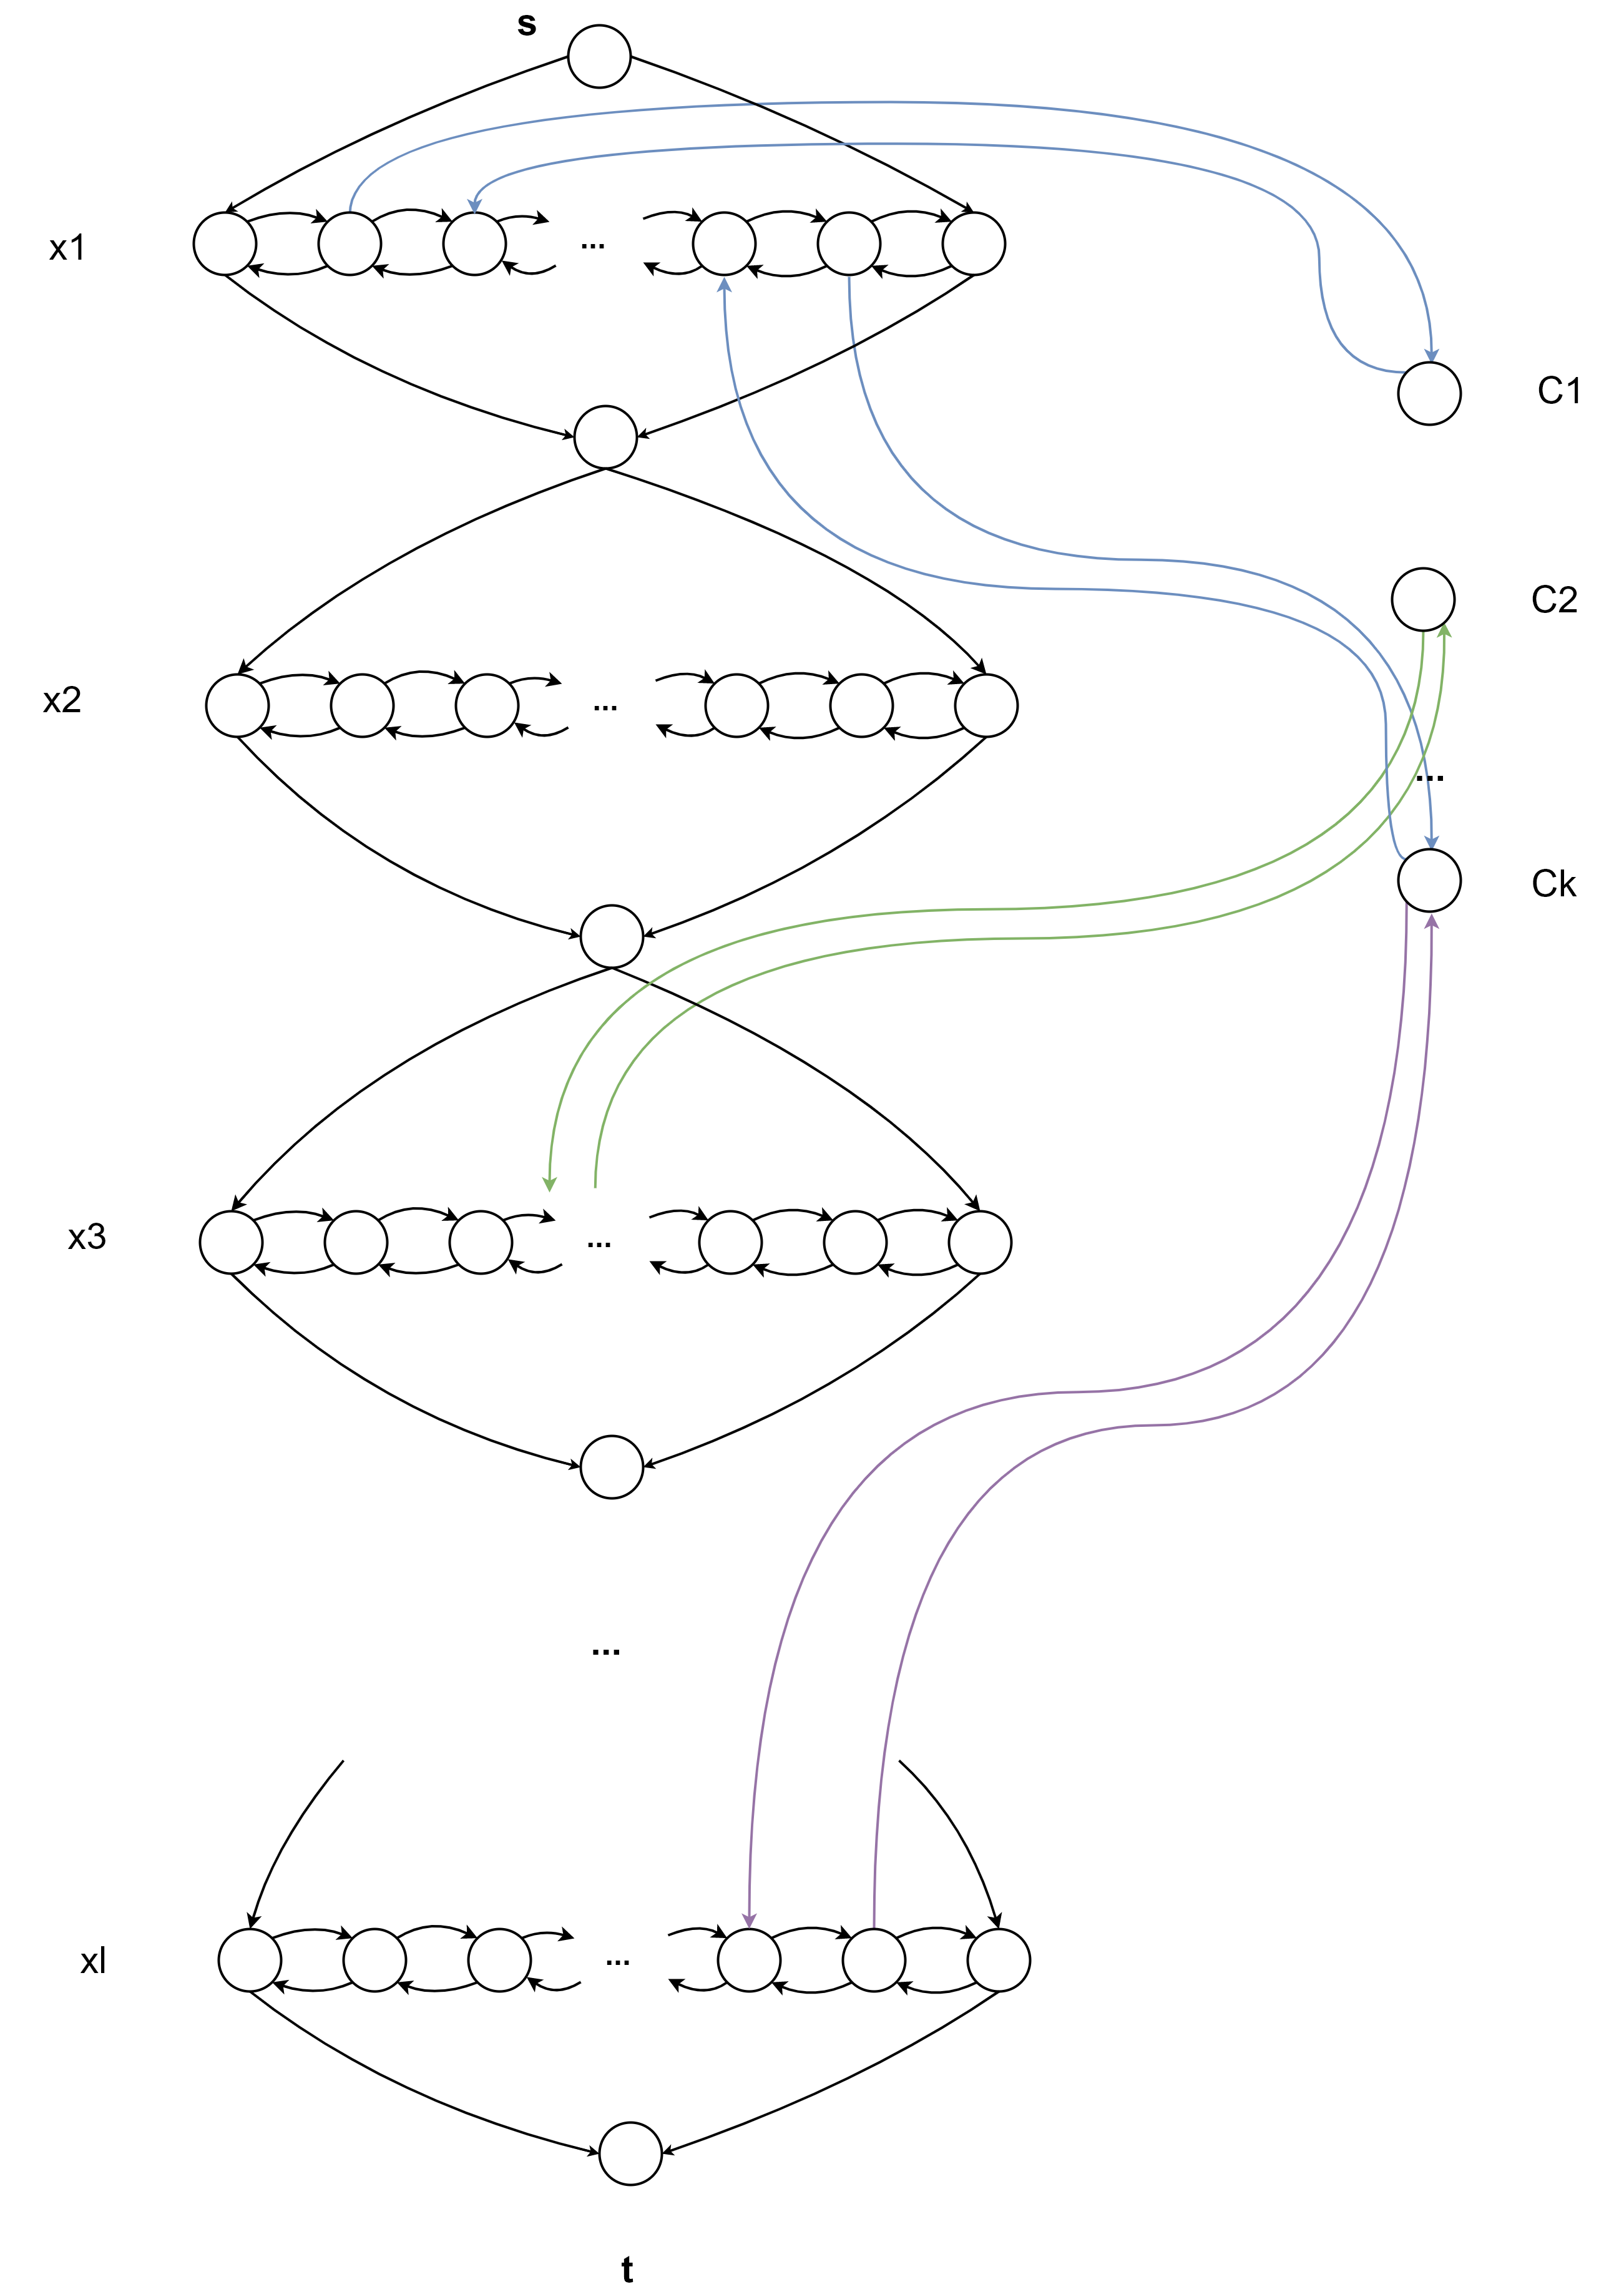
\includegraphics[scale=0.15]{3.png}\\
那么如果在此图中找到了一条Hamilton路径,可以确定一种x的赋值:若此路径从第i个钻石子图的左边进入,右边离开,$x_i$赋值为1,否则为0,并且此种赋值可以满足表达式。\\
显然,这种转化可以在$\mathcal{O}(k)$的时间完成,若找到了Hamilton路径,表达式结果为1,结果转换是$\mathcal{O}(1)$,因此Hamilton路径问题是NP-hard问题。
\section{}
题目:在瓶颈旅行商问题中,目标是找出这样一条哈密顿回路, 使得回路中代价最大的边的代价相对于其他回路来说最小。假设代价函数满足三角不等式,证明:这个问题存在一个近似比为 3 的多项式时间近似算法。

证明:\\
给出多项式算法:\\
(1)随机选一个结点1作为回路起点和终点\\
(2)从起点开始,利用Prim算法计算该图的最小生成树\\
(3)从起点开始先序遍历最小生成树,依次打印遍历结果,打印完毕后在最后添加起点1作为终点\\
证明此算法为近似比为3的多项式时间近似算法:\\
(1)设最小生成树各边的权重之和为$cost_{MST}$,那么有$cost_{best}>cost_{MST}$\\
(2)设遍历最小生成树的过程中,走过的边(算上重复走的)的权重总和为$cost_{MST}'$,那么有$2*cost_{MST}<cost_{MST}'$\\
(3)设由算法给出的近似解的总代价为$cost_{algo}$,那么由三角不等式,有$cost_{algo}<cost_{MST}'$\\
因此,$cost_{algo}<2*cost_{best}<3*cost_{best}$,所以算法是近似比为3的多项式时间近似算法。
\section{}
题目:设 G = (V,E) 是一个无向图,其中是每条边$(u,v)\in E$具有不同的权值$\omega(u,v)$。对每个顶点$v\in V$,设$\max{v}=argmax_{(u,v)\in E}\{\omega(u,v)\}$是与顶点$v$相关联的最大权值边。设$S_G=\{max(v):v\in V\}$表示与各个顶点相关联的最大权值边的集合,$T_G$表示图$G$的最大权值生成树。对任意的边集$E'\subseteq E$,定义$\omega(E')=\sum_{(u,v)\in E'}\omega(u,v)$。
\subsection{a. 给出一个至少包含 4 个顶点的图,使其满足 $S_G = T_G$。}
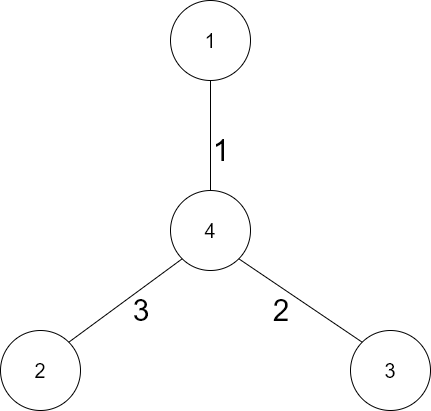
\includegraphics[scale=0.3]{4.png}
\subsection{b. 给出一个至少包含 4 个顶点的图,使其满足 $S_G\neq T_G$。}
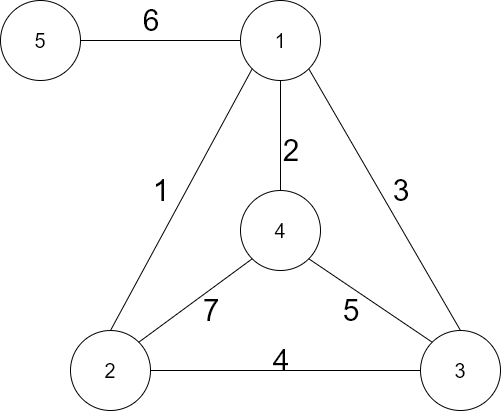
\includegraphics[scale=0.3]{5.png}
\subsection{c. 证明:对任意的图 G,$S_G \subseteq T_G$。}
利用反证法:\\
若$\exists(u,v)\in S_G$且$(u,v)\notin T_G$,令$(u,v)=\max{(u)}$\\
选择,$T_G$中,与$u$相连的,在当前的生成树中处于u到v的路径上的唯一边$(u,v')$(显然,生成树中u到v的路径唯一,若不唯一,则有环,所以$(u,v')$唯一),若用$(u,v)$代替$(u,v')$,即将$(u,v')$从$T_G$中删去,将$(u,v)$加入$T_G$,得到了权值更大的生成树,与$T_G$是最大权值生成树相矛盾。故不存在一条属于$S_G$但不属于$T_G$的边,即$S_G\subseteq T_G$
\subsection{d. 证明:对任意的图$G$,$\omega(T_G)\geq \omega(S_G)/2$}
由c问,可知$S_G\subseteq T_G$,那么有$\omega(T_G)\geq \omega(S_G)$,即有$\omega(T_G)\geq \omega(S_G)/2$
\subsection{e. 给出一个$\mathcal{O}(V+E)$时间算法,用于计算 2 近似的最大生成树。}

\floatname{algorithm}{Algorithm}
\renewcommand{\algorithmicrequire}{\textbf{输入:}}
\renewcommand{\algorithmicensure}{\textbf{输出:}}
\begin{algorithm}
	\caption{}
	\begin{algorithmic}[1]
	\Require 图G
	\Ensure 近似最大生成树$T_G$
	\For{$each\ vertex\ v\ \in G.V$}
		\State{v.max = max(v)}
		\State{$T_G$ += v.max}
	\EndFor
	\While{$T_G.size\ <\ |G.V|-1$}
		\State{Find (u,v) not in $T_G$ and weigh max and no circle if add to $T_G$}
		\State{$T_G$ += (u,v)}
	\EndWhile\\
	\Return (u,v)
	\end{algorithmic}
\end{algorithm}
此算法可以计算2近似的最大生成树,因为此算法以$S_G$为基础寻找$T_G$。\\由$S_G$性质可知,$|S_G|\geq |G.V|/2$,又由c问$S_G\subseteq T_G$。按照最坏的情况考虑,若$|S_G|=|G.V|/2$,$S_G$将$T_G$分成了$S_G$和$T_G-S_G$两个集合,在这种情况下$|T_G-S_G|=|G.V|/2-1$,那么一定有$\omega(S_G)>\omega(T_G-S_G)$,有由于$\omega(S_G)+\omega(T_G-S_G)=\omega(T_G)$,所以$\omega(S_G)>\omega(T_G)/2$,因此此算法可以解得2近似的最大生成树。
\section{给出一种 2-SAT 问题的多项式解法。}
\floatname{algorithm}{Algorithm}
\renewcommand{\algorithmicrequire}{\textbf{输入:}}
\renewcommand{\algorithmicensure}{\textbf{输出:}}
\begin{algorithm}
	\caption{}
	\begin{algorithmic}[1]
	\Require 布尔表达式F
	\Ensure 此表达式是否可满足
	\For{each clause in F (x1,x2)}
		\State{//x and /x is not the same node}
		\If{x1's node is not in graph G}
			\State{add a node named x1 into G}
			\State{add a node named /x1 into G}
		\EndIf
		\If{x2's node is not in graph G}
			\State{add a node named x2 into G}
			\State{add a node named /x2 into G}
		\EndIf
		\State{add edge (/x1,x2)}
		\State{add edge (/x2,x1)}
	\EndFor
	\If{DFSFindStronglyConnectedComponet(G)}\\
		\quad\quad\Return False
	\Else\\
		\quad\quad\Return True
	\EndIf
	\end{algorithmic}
\end{algorithm}

\end{document}
